\documentclass[]{report}
\usepackage[hmargin=1.25in,vmargin=1in]{geometry} %调整页边距
% \usepackage[inner=1in,outer=1.25in]{geometry} %书籍左右不等宽排版
\usepackage[utf8]{inputenc}
\usepackage[]{ctex} %据说可以直接调用诸如 \kaishu \fangsong \heiti 的命令修改字体
\usepackage[svgnames]{xcolor} % Using colors
% \usepackage{background} % To include background images
\usepackage{fancyhdr} % Needed to define custom headers/footers
\usepackage[]{xeCJK}
\setCJKmainfont[BoldFont = STHeiti, ItalicFont = STKaiti]{Songti SC Light} %中文主字体
\setCJKsansfont[BoldFont = Weibei SC, ItalicFont = HanziPen SC]{Xingkai SC Light} %中文无衬线字体
\setCJKmonofont[BoldFont = Libian SC, ItalicFont = STFangsong]{Yuanti SC Light} %中文等宽字体
\setmainfont{Times New Roman} %\rmfamily
\setsansfont[ItalicFont = American Typewriter]{Comic Sans MS} %\sffamily
\setmonofont{Courier} %\ttfamily
\renewcommand{\emph}[1]{\textbf{\textit{#1}}}
\usepackage{titlesec}
\titleformat{\chapter}{\centering\huge\bfseries}{第~\thechapter~部分}{1em}{}

\usepackage{ulem} %解决下划线、删除线之类的
\usepackage{listings}
\lstset{
language=C++,
keywordstyle = \color{blue}\bfseries,
commentstyle=\color{green},
tabsize = 4,
%backgroundcolor=\color{bg}
emph = {int,float,double,char},emphstyle=\color{cyan},
emph ={[2]const, typedef},emphstyle = {[2]\color{red}} }

\usepackage{amsmath} %数学公式问题
\usepackage{amsthm} %公式环境,如proof
\usepackage{booktabs} %三线表
\newcommand{\tabincell}[2]{\begin{tabular}{@{}#1@{}}#2\end{tabular}} %解决单元格内部换行的问题
% 比如这个 Beijing & 0,5 & 1,6 & 2,7 & 3,8 & 4,9 & The number changes every 3 months \\
% 改成这个 \tabincell{l}{Beijing}& \tabincell{c}{0,5}& \tabincell{c}{1,6}& \tabincell{c}{2,7}& \tabincell{c}{3,8}& \tabincell{c}{4,9}& \tabincell{c}{The number changes \\ every 3 months} \\
% 一个单元格过长,整行都需要修改
% 可以配合 \resizebox*{h-width}{v-width}{contents, e.g.tabular} 使用

\usepackage{mathrsfs} %在公式里面使用那个最花的字体
\usepackage{amssymb} %公式里面用空心黑体和旧式字体
\usepackage{amssymb} %AMS符号
\usepackage{amsthm} %AMS定理环境

\usepackage{markdown} %使用markdown语法,在编译时需要打开 shell-escape 标记,即 $ xelatex --shell-escape example.tex
\markdownSetup{hashEnumerators = true} %允许使用 #. 的方式编写有序列表
\markdownSetup{inlineFootnotes = true} %允许使用脚注形式的超链接,调用语法为 [anchor](uri), ^[footnote], <uri>
\markdownSetup{fencedCode = true} %以反引号和缩进来插入代码段,相当于 verbatim
\markdownSetup{
  pipeTables = true
} %支持表格的用法 (图片已经在markdown包里面支持了)
% \usepackage{booktabs} %解决三线表的线条粗细问题

\usepackage{graphicx} %插入图片
\usepackage{pdfpages} %插入PDF文件
\usepackage{makeidx}

\usepackage{tikz} %带圈字符
\usepackage{etoolbox} %带圈字符 (提供robustify)
\usepackage{enumitem}
\newcommand*{\circled}[1]{\lower.7ex\hbox{\tikz\draw (0pt, 0pt)%
    circle (.5em) node {\makebox[1em][c]{\small #1}};}} %新定义命令:带圈字符
\robustify{\circled}
% \usepackage{enumerate} %有序列表

\usepackage{hyperref} %超链接
% \usepackage[hidelinks]{hyperref} %隐藏超链接的红框
\markdownSetup{
  inlineFootnotes = true,
  renderers = {
    link = {\href{#3}{#1}},
  }
} % markdown块中使用直接点进去的超链接
% \setlist[enumerate,1]{label=(\arabic*).,font=\textup,leftmargin=7mm,labelsep=1.5mm,topsep=0mm,itemsep=-0.8mm}
% \setlist[enumerate,2]{label=(\alph*).,font=\textup,leftmargin=7mm,labelsep=1.5mm,topsep=-0.8mm,itemsep=-0.8mm}

\usepackage{braket}

%%%%%% Setting up the style

% \setlength\parindent{0pt} % Gets rid of all indentation
% \backgroundsetup{contents={\includegraphics[width=\textwidth]{ustc-name.pdf}},scale=0.4,placement=top,opacity=0.6,color=cyan,vshift=-20pt} %  USTC Logo

\pagestyle{fancy} % Enables the custom headers/footers

% Use default headers
% \lhead{} \rhead{} % Headers - all  empty

% \title{\vspace{-1.8cm}  \color{DarkRed} Laboratory Rotation Report}
% \subtitle{Title of the proposal % Title of the rotation project
% \vspace{-2cm} }
% \date{\today} % No date

\lfoot{\color{Grey} \textit{上官凝}}  % Write your name here
\rfoot{ \color{Grey} \texttt{\textit{运筹学基础复习笔记}} }
\cfoot{\color{Grey} \thepage}

\renewcommand{\headrulewidth}{0.0pt} % No header rule
\renewcommand{\footrulewidth}{0.4pt} % Thin footer rule

\title{运筹学基础笔记}
\author{上官凝}
\date{\today}

\linespread{1.3} %行间距为1.3倍默认间距 (1.3 x 1.2倍字符宽度)

\makeindex

\begin{document}
\theoremstyle{definition} \newtheorem{theorem}{Thm}[section] %定义一个定理Thm,序号为section的下一级序号
\theoremstyle{definition} \newtheorem{definition}{Def}[section] %定义一个定义Def,序号为section的下一级序号
\theoremstyle{plain} \newtheorem{lemma}{lemma}[section] %引理

	\maketitle
	\newpage

	\tableofcontents
	\newpage

	\section{序幕}
	% \textit{风乍起,吹皱一池秋水}\par
	{\Large{最优解一定是可行解,未必是基解}}\par
	这门课就是叫你算,算足一百八十天,算出美味算出鲜!\footnote{更多内容请移步评课社区}\par
	总体上来讲,单纯形法的思路都是一致的,即通过换入变量和换出变量的代换,循环迭代最终得到最优解,或者无穷多最优解、无界解、无可行解的结论。方程组形式的单纯形法为所有变种的来源,后续方法进行简化或者应对特别的问题进行变化。在解题过程中,一定要多考虑是否已经可以看出为无可行解,可以避免耽误时间\par
	分析问题很重要,因为很有可能第一眼看到的不是这题真正想要考的,比如下面这个题(P109\ 例4)\par
	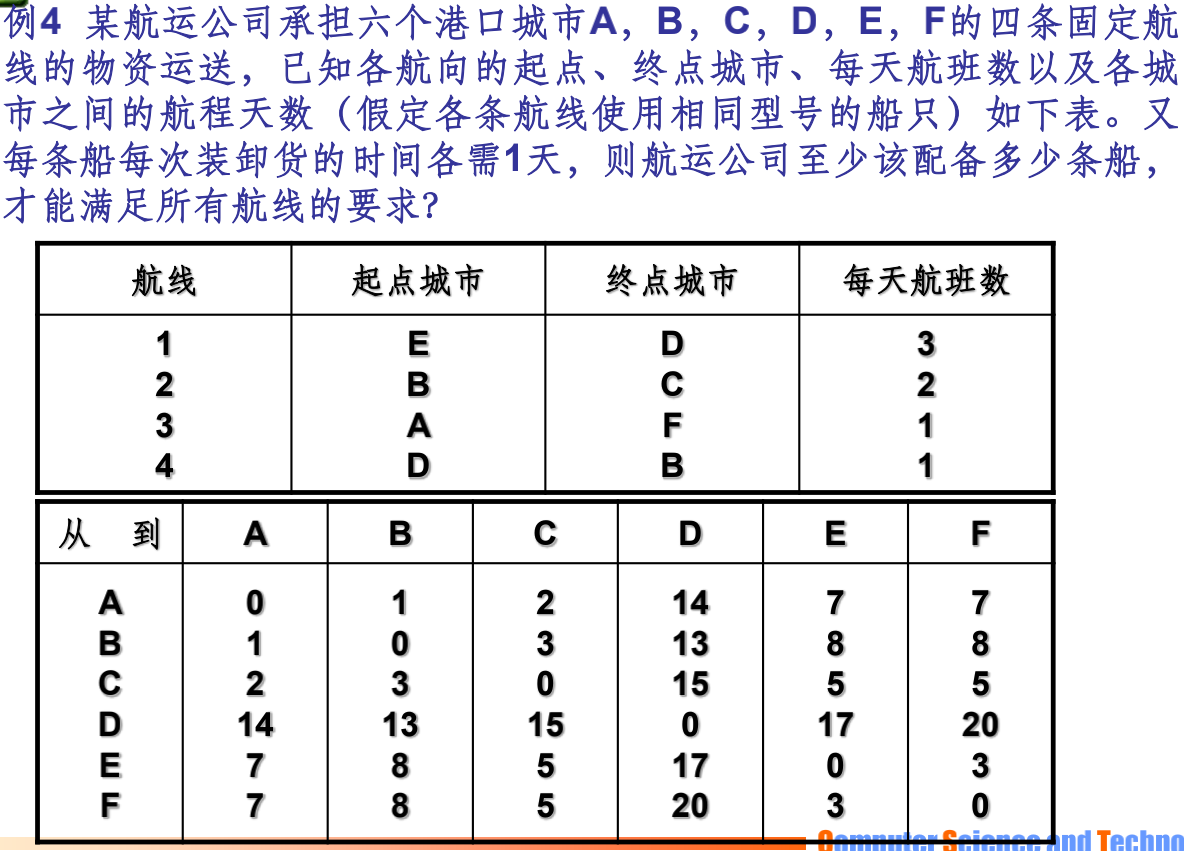
\includegraphics[scale = 0.3]{pictures/P109_Example4.png}\par

	\newpage
	% \includepdf[pages={1,2,3,4,5,6,7,8}]{ref_files/or_elemen.pdf}
	% \includegraphics[scale = 0.8]{ref_files/or_elemen.pdf}
	% \chapter{各章节知识整理}
	% 此部分为笔者的学习笔记,主要从GNJ教授的PPT上摘抄而来,如有疏漏或错误,欢迎提issue
	% \newpage
	% \begin{markdown}
	% 	\include{ref_files/OR_notes.md}
	% \end{markdown}
	% % \includepdf[pages={1,2}]{or_elemen.pdf}
	% \newpage
	% \section{第二章 线性规划及单纯形法}
	% \subsection{Cautions:}
	% \begin{enumerate}
	% 	\item 拿到一个线性规划问题之后,先把它化为标准型
	% 	\item 可行解与最优解:满足约束条件的解为可行解,使目标函数达到最大的可行解为最优解
	% 	\item 单纯形法的变量定义:决策变量 $x_{j}$,价值系数 $c_j$,技术系数 $a_{ij}$,限额系数 $b_i$
	% \end{enumerate}

	\chapter{对一些知识点的探讨}
	\section{关于单纯形表法和普通单纯形法}
	我个人的习惯是列出来一个单纯形表(至少写成增广矩阵)看起来要比用线性方程组要直观一些,对于每一步的$\sigma,\ \theta$的求解会清晰一点\par
	\textbf{P.S.}一定一定要记得使全部$\boldsymbol{b}$为\textbf{正的!正的!正的!}
		\subsection{关于线性规划问题的标准化}
		标准化的一个目的是找出一组基变量。首先(我的习惯是)目标函数变成$\max z$的形式,若为求最小值,则令$w=-z$即可。其次需要满足限额系数$b_i>0$。每一个约束方程都可以是等式或者不等式,若为等式,则可以用高斯消元的思想来得到基变量,或者采取增加人工变量的方式;若为$\le$,则添加的松弛变量即为该行的基变量;若为$\ge$,则在添加剩余变量之后,仍需添加人工变量来构造一组基解。采用人工变量的目的是采取一个较为通用的办法来找出一组初始的可行基,我个人认为最好写上\textbf{M为无穷大正数}

		\subsection{关于换入变量以及换出变量的确定}
		一定要注意一些先决条件,而不是一上来就直接算一个$\max\sigma_j$,再算一个$\min\theta_k$。可能会出现以下情况(可能没有列举全):\par
		\begin{enumerate}
			\item 检验数只算非基变量,所以搞清楚哪几个是真正的非基变量,尤其在矩阵法计算和运输问题等变量的表述较为隐蔽的情形下
			\item $\theta$规则只在对应列正的技术系数$a_{ij}$之间比较
			\item 关于Blend法则:当$\sigma$或$\theta$ 规则计算时,有两个以上的最小相同比值,选取 $c_j-z_j$ 中下标最小的 $\Rightarrow$ 换入变量,选取 $\theta$ 比值中下标最小的 $\Rightarrow$ 换出变量
			\item 线性目标规划由于在不同决策变量之间存在优先级,故在高优先级的检验数行不全为0时,毋需计算和考虑低优先级检验数行
		\end{enumerate}

		\subsection{线性规划问题的BreakOut点}
		对于一个普通的标准型,有以下情形;对于后面几章拓展的线性规划问题,在形式上参照下表
		\begin{enumerate}
			\item 存在最优解:所有非基变量的检验数均小于0
			\item 存在无穷多解:所有非基变量的检验数均小于等于0,且存在某个非基变量的检验数等于0
			\item 存在无界解:有一个非基变量的检验数大于0,且这一列的技术系数都小于等于0
			\item 无可行解:(在添加人工变量之后,才有可能出现无可行解)存在未换出的人工变量、或两阶段法的第一段最优解不为0
		\end{enumerate}
		\subsection{人工变量的两阶段法}
		第一阶段:不考虑原问题是否存在基可行解;给原线性规划问题加入人工变量,并构造仅含人工变量的目标函数和要求实现最小化。如将目标函数修改为 $\min w=x_{n+1}+\cdots+x_{n+m}+0x_1+\cdots+0x_n$,然后用单纯形法求解上述模型,若得到$w=0$,这说明原问题存在基可行解,可以进行第二段计算,否则无可行解\par
		第二阶段:将第一阶段得到的最终表,除去人工变量的列,目标函数换回原来的
	\section{关于丹齐克的改进单纯形法}
	\texttt{改进单纯形法每一步所乘上的b 和 N 均直接从约束条件而非上次计算得}\par
		\subsection{关于矩阵方法计算的一点理解}
		改进单纯形法是借助矩阵来运算的,其改进的核心是不需要像单纯形表一样每一次迭代都需要计算出来基变量矩阵$B$,而是由于公式$B_{n}^{-1}=EB_{n-1}^{-1}$这样一个推导公式,直接计算$B^{-1}$便可以进入下一轮迭代。由于矩阵表示隐藏了原单纯形表的内部结构,故理解起来或许稍有困难,加以PPT写的又不甚清楚,故笔者在此参考\href{https://zhuanlan.zhihu.com/p/65512496}{知乎上一篇文章}中的部分文字加以解释\par
		首先让我们来看线性代数里矩阵初等行变换的三种形式:\footnote{《线性代数与解析几何 第二版》陈发来等编,102页}\par
		\begin{enumerate}[label = (\arabic{*})]
			\item 交换矩阵的两行
			\item 将某行乘以一个非零常数
			\item 将某行的常数倍加到另一行
		\end{enumerate}\par
		回忆一下,单纯形表的计算是不是就是这三种?再由线性代数定理4.4.1:\textit{对矩阵做初等行变换,相当于在矩阵的左边乘上一个相应的初等方阵;对矩阵做初等列变换,相当于在矩阵的右边乘上一个初等方阵} 可知,对单纯形表进行变换时,实则是在对单纯形表的那个矩阵进行一次次的初等行变换,也是在用一个又一个的初等矩阵左乘该矩阵。而这个矩阵,便是在第i轮迭代中的$B_i^{-1}$\par
		回想单纯形表年代每一轮迭代的三步计算:\par
		$$\begin{aligned}
			\sigma_j=c_j-\sum_{i=1}^mc_ia_{ij},\\
			\theta=\frac{b_i}{a_{ik}},\\
			make\ out\ next\ table
		\end{aligned}$$
		对比二者公式,可以发现每一步矩阵方法多了一个左乘$B_{-1}$,而结合前文所述,左乘正是为了得到单位阵化之后的基变量矩阵(我尽可能的说清楚\textsf{\textit{QAQ}},如有不清晰的请告诉我或者画一个图理解一下\dots)

		\subsection{关于迭代矩阵E的计算}
		\[E=\begin{pmatrix}
			e_1,\cdots,e_{l-1},\xi,e_{l+1},\cdots,e_m
		\end{pmatrix}\]
		\[\xi=\begin{pmatrix}
			-a_{1k}/a_{lk},\cdots,1/a_{lk},\cdots,-a_{mk}/a_{lk}
		\end{pmatrix}^{\mathrm{T}}\]
		可见,转换矩阵在行和列的定位都是依靠换出变量的排序下标$l$,而换入变量的下标$k$只在取$a_{lk}$时用到,转换矩阵的对角线上$(l,l)$位置便是最特殊的一个位置(个人理解)。\textbf{需要注意的是},这些技术系数是在第n步中单纯形表里面的系数,即当前的$B_{n}^{-1}\cdot P_i$,以下面这个题为例说明一下(87页 3.1(2))\par
		\paragraph{例} 用改进单纯形法求解以下线性规划问题\[\min z=2x_1+x_2\]\[\begin{cases}
			3x_1+x_2=3\\
			4x_1+3x_2\ge6\\
			x_1+2x_2\le3\\
			x_1,x_2\ge0
		\end{cases}\]
		\paragraph{解} 化为如下形式(不是标准型)\[\min z=2x_1+x_2+Mx_3+0x_4+Mx_5+0x_6\]\[\begin{cases}
			3x_1+x_2+x_3=3\\
			4x_1+3x_2-x_4+x_5=6\\
			x_1+2x_2+x_6=3\\
			x_1,x_2,x_3,x_4,x_5,x_6\ge0
		\end{cases}\]其中M为任意大正数,则在迭代一次之后得到:
		\[X_{B_1}=(x_1,x_5,x_6)^{\mathrm{T}}\qquad X_{N_1}=(x_3,x_2,x_4)^{\mathrm{T}}\]
		\[C_{B_1}=(2,M,0)\qquad C_{N_1}=(M,1,0)\]
		\[B_1^{-1}=\begin{pmatrix}
			\frac{1}{3}&0&0\\
			-\frac{4}{3}&1&0\\
			-\frac{1}{3}&0&1
		\end{pmatrix}\]
		\[\sigma_1=(-\frac{2}{3}+\frac{7}{3}M,\frac{1}{3}-\frac{5}{3}M,M)\]
		故$x_2$为换入变量
		\[\theta=\min\left\{\frac{(B_1^{-1}b)_i}{(B_1^{-1}P_2)_i}\mid(B_1^{-1}b)_i>0\right\}=\min\left\{3,\frac{6}{5},\frac{6}{5}\right\}=\frac{6}{5}\]
		由Blend法则确定出$x_5$为换出变量\par
		\textsf{\textit{注意这一块}}
		\[B_1^{-1}P_2=\left(\frac{1}{3},\frac{5}{3},\frac{5}{3}\right)^{\mathrm{T}}\]
		\[\xi=\left(-\frac{\frac{1}{3}}{\frac{5}{3}},\frac{3}{5},-\frac{\frac{5}{3}}{\frac{5}{3}}\right)^{\mathrm{T}}\]
		\[E=\begin{pmatrix}
			1&-\frac{1}{5}&0\\
			0&\frac{3}{5}&0\\
			0&-1&1
		\end{pmatrix}\]
		\[B_2^{-1}=E\cdot B_1^{-1}=\begin{pmatrix}
			\frac{3}{5}&-\frac{1}{5}&0\\
			-\frac{4}{5}&\frac{3}{5}&0\\
			1&-1&1
		\end{pmatrix}\]
		\textsf{\textit{在计算迭代矩阵的时候可能出现的坑:}}\par
		有可能会有这一次迭代的中心位置在初始问题中为0,导致计算迭代矩阵的时候出现分母为0的情况。说起来有点抽象,参考下例(page 87,习题3.1):
		\paragraph{例} 用改进单纯形法求解以下线性规划问题\[\max z=6x_1-2x_2+3x_3\]\[\begin{cases}
			2x_1-x_2+2x_3\le2\\
			x_1+4x_3\le4\\
			x_1,x_2,x_3\ge0
		\end{cases}\]在第二次迭代时,换入变量为$x_2$,换出变量为$x_5$,而此处对应的原始的值为0。可以采取的方案是直接求出B,然后待定系数求$B^{-1}$

		\subsection{关于本部分一些非常规的解题}
		\textit{参考《运筹学 第四版》清华大学出版社,P89 习题3.7}\par
		灵活运用矩阵法求解的本质思想,即单纯形法求解线性规划问题的本质是在增广矩阵上做初等行变换;以及一些小的结论,
		3.7题如图所示:\par
		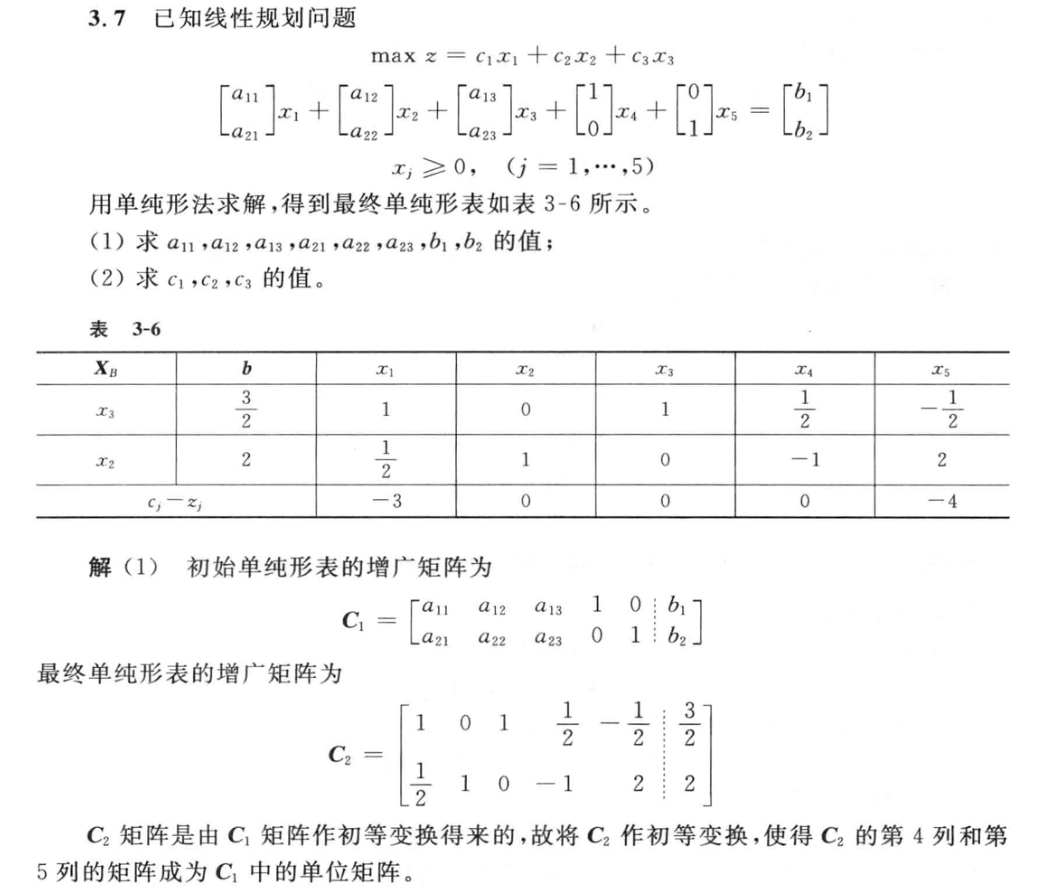
\includegraphics[scale = 0.37]{pictures/Exe_3.7.png}\par
	\section{关于对偶单纯形法}
		对偶单纯形法最大的优点为原问题的初始解不一定是基可行解(免去了人工变量法),可以从非基可行解开始迭代;同时其缺点是大多数情况下很难找到一个初始可行基。普通单纯形法对检验数为$\sigma_N=c_N-c_BB^{-1}N$,即使用价值系数来进行判断;而对偶单纯形法则是用$B^{-1}b$,即使用限额系数来进行判断
		\subsection{对偶问题}
		对偶单纯形法基于对原线性规划问题的对偶问题对求解。在求解对偶问题时,应当注意以下两点:
		\begin{enumerate}
			\item 并没有规定原问题就必须是$\max z$,转换表双向都是可以的
			\item 但是两个方向规则不是完全相同的,$\max$到$\min$的转换,变量到约束条件不等号方向不变;而$\min$到$\max$的转换,变量到约束条件不等号方向要改变(请对照前文转换表,会更直观一些)
		\end{enumerate}

		\subsection{对偶问题性质的应用}
		在证明中较为重要的性质有二:
		\begin{enumerate}
			\item 弱对偶性:原问题的可行解 $\overline{X}$,对偶问题可行解 $\bar{Y}$,则 $C\overline{X}\leq\overline{Y}b$,取等时同时达到最优解
			\item 对偶定理:若原问题有最优解,那么对偶问题也有最优解,且目标函数值相等
		\end{enumerate}
		现举一例以言之\footnote{《运筹学 第四版》清华大学出版社,P89 习题3.5}:\par
		\paragraph{例}
		设线性规划问题1是
		$$\max z_1=\sum_{j=1}^nc_jx_j$$
		$$\begin{cases}
			\sum_{j=1}^na_{ij}x_j&\le b_i,\quad i=1,2,\cdots,m\\
			x_j\ge0,\quad &i=1,2,\cdots,n
		\end{cases}$$
		$(y_1^*,\cdots,y_m^*)$是其对偶问题的最优解,又设线性规划问题2是
		$$\max z_2=\sum_{j=1}^nc_jx_j$$
		$$\begin{cases}
			\sum_{j=1}^na_{ij}x_j\le b_i+k_i,\quad &i=1,2,\cdots,m\\
			x_j\ge0,&i=1,2,\cdots,n
		\end{cases}$$
		其中$k_i$为给定的常数,求证$\displaystyle\max z_2\le\max z_1+\sum_{i=1}^mk_iy_i^*$\par
		\begin{proof}
			将二者的原问题用矩阵形式描述如下:
			$$\max z_1=CX$$
			$$\begin{cases}
				AX\le\boldsymbol{b}\\
				X\ge0
			\end{cases}$$
			并设其可行解为$X_1$,对偶问题的最优解$Y_1$为已知\par
			$$\max z_2=CX$$
			$$\begin{cases}
				AX\le\boldsymbol{b}+\boldsymbol{k}\\
				X\ge0
			\end{cases}$$
			并设其可行解为$X_2$,对偶问题的最优解$Y_2$,其对偶问题为\par
			$$\min w_2=Y(\boldsymbol{b}+\boldsymbol{k})$$
			$$\begin{cases}
				YA\ge C\\
				Y\ge0
			\end{cases}$$
			因为$Y_2$为最优解,故$Y_2(\boldsymbol{b}+\boldsymbol{k})\le Y_1(\boldsymbol{b}+\boldsymbol{k})$\par
			因为$X_2$为第二个线性规划问题的可行解,故$AX_2\le\boldsymbol{b}+\boldsymbol{k}$,故$Y_2AX_2\le Y_2(\boldsymbol{b}+\boldsymbol{k})\le Y_1(\boldsymbol{b}+\boldsymbol{k})$\par
			因为原问题与对偶问题的最优函数值相等(因为$Y_2$是最优解?),故$Y_2A\ge C$\par
			(或者由弱对偶性得到$CX_2\le Y_2(\boldsymbol{b}+\boldsymbol{k})$)\par
			故$CX_2\le Y_2AX_2\le Y_2(\boldsymbol{b}+\boldsymbol{k})\le Y_1(\boldsymbol{b}+\boldsymbol{k})$
		\end{proof}

		\subsection{互补松弛性解题}
		互补松弛性:$\hat{Y}X_S=0$且$Y_S\hat{X}=0\Leftrightarrow\hat{X},\hat{Y}$ 为优解,其中 $\hat{X},\hat{Y}$ 分别为原问题、对偶问题的可行解(习题3.8)\par
		互补松弛性大前提是原问题与对偶问题都取可行解。将两个问题添加上松弛变量与剩余变量得到等式约束。比如现有对偶问题Y的一组可行解,那么就有$\hat{Y}X_S=0$、$Y_S\hat{X}=0$和$AY+Y_S=b_Y=C$三组矩阵方程,对这些方程加以分析与解可以得到结果

		\subsection{关于对偶单纯形法本身}
		明确一下对偶单纯形法和普通单纯形法的几个不同点:(按照对偶单纯形法的操作步骤来说)\par
		\begin{enumerate}
			\item 对偶单纯形法一上来要对原有单纯形表进行变换,使列出的初始单纯形表所有检验数$\sigma_j ≤ 0,\,(j=1,2,…,n)$,即对偶问题为基可行解(单纯形法此处要求所有$b_i\ge0$)
			\item 检查 b 列,若都非负,又检验数为非正,则得到最优解;若b列存在负分量,继续(单纯形法是观察检验数是否全为非正)
			\item 确定换出变量:按照 $\min\{(B^{-1}b)_i\mid(B^{-1}b)_i<0\}=(B^{-1}b)_l$ 来确定 $x_l$ 为换出变量(普通单纯形法是先确定换出变量再确定换入变量,且注意不等号方向,这两步大于小于0都有所差异)
			\item 确定换入变量:检查 $x_l$ 所在行的系数,若都大于0,则无可行解;反之按照$\theta$规则 $\displaystyle\theta=min(\frac{c_j-z_j}{a_{lj}}\mid a_{lj}<0)=\frac{\sigma_k}{a_{lk}}$ 来确定换入变量
		\end{enumerate}\par
		\begin{figure}[h]
			\centering
			\begin{minipage}{40em}
				\centering
				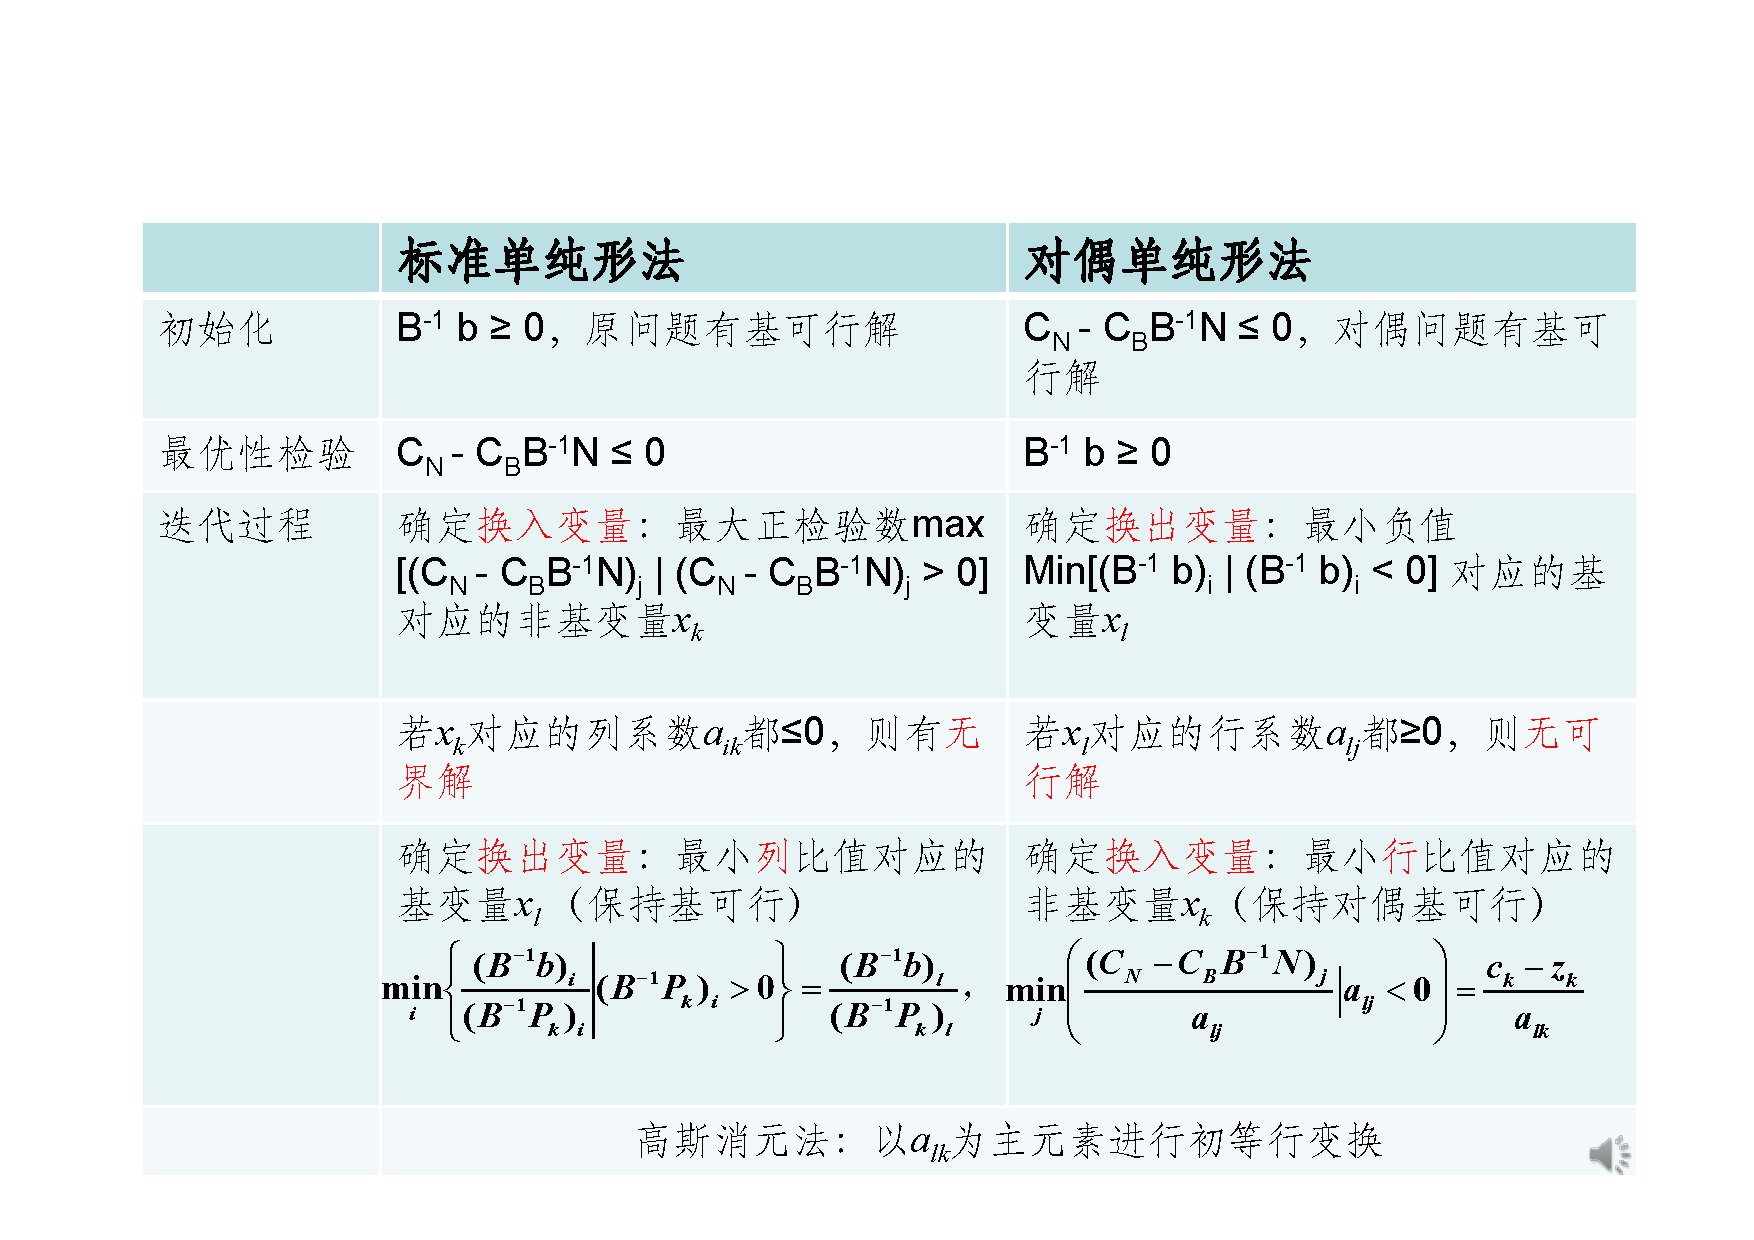
\includegraphics[scale = 0.5]{pictures/DanChunXingFa.pdf}
				\caption{对偶单纯形法与普通单纯形法的比较}
			\end{minipage}
		\end{figure}\par
	\section{关于灵敏度分析}
		也称为敏感性分析,它是研究和分析参数$(c_j,b_i,a_{ij})$的波动对最优解的影响程度,主要研究下面两个方面:\par
		\begin{enumerate}
			\item 参数在什么范围内变化时,原最优解或最优基不变
			\item 当参数已经变化时,最优解或最优基如何变化
		\end{enumerate}\par
		当模型的参数发生变化后,可以不必对线性规划问题重新求解, 而用灵敏度分析方法直接在原线性规划取得的最优结果的基础上,进行分析或求解,既可减少计算量,又可事先知道参数的变化范围,及时对原决策作出调整和修正\par
		\begin{table}[h]
			\centering
			\begin{tabular}{ccc}
				\toprule
				原问题 & 对偶问题 & 结论或继续计算的步骤\\
				\midrule
				可行解   & 可行解   & 表中的解仍为可行解\\
				可行解   & 非可行解 & 用单纯形法迭代求最优解\\
				非可行解 & 可行解   & 用对偶单纯形法迭代求最优解\\
				非可行解 & 非可行解 & 引入人工变量,编制新的单纯形表求最优解\\
				\bottomrule
			\end{tabular}
		\end{table}\par
		总体上的思路都是判断变换之后的问题是不是依然满足非基变量检验数非正,若不满足则需要继续单纯形迭代。下面是整理一下这部分具体的知识点(其实我觉得不用记公式,用原理判断要更好记:\par
		\begin{enumerate}
			\item $b_i$:保证$X_B'=B^{-1}(\boldsymbol{b}+\Delta\boldsymbol{b})>0$,不满足用对偶单纯形法(因为$\boldsymbol{b}$改变了有可能会出现小于0)
			\item $c_i$:保证这个价值系数影响到的检验数都非正,若不然则采用单纯形法(同样,因为有可能检验数破坏了对偶可行性)
			\item 增加一个变量:保证这个变量的检验数非正,否则采用单纯形法
			\item 增加一个约束条件:增加松弛变量(对偶单纯形法)或人工变量法
			\item $x_{ij}$:见下方具体解析
		\end{enumerate}
		\subsection{可以直接作出判断的结论,以及变化之后的调整策略}
		简要列出来一些可以直接作出判断的结论,以供参考。一定要先判断是不是维持原有最优基不变,真的不要像一个铁憨憨似的上来就对偶单纯形法暴算\dots
			\paragraph{资源数量$b_i$}\par
			改变:$\boldsymbol{b}$中的第r项$b_r'=b_r+\Delta b_r$\par
			最优基不变范围:$\max\{-\bar{b}_i/\bar{a}_{ir}\mid\bar{a}_{ir}>0\}<\Delta b_r<\min\{-\bar{b}_i/\bar{a}_{ir}\mid\bar{a}_{ir}<0\}$,其中$\bar{b}_1$指原来线性规划问题解出来的最优解基变量的第i项,而$\bar{a}_{ir}$指矩阵$B^{-1}$中的第$(i,r)$位置的元素\par
			若不符合不变条件,则在原有问题最终单纯形表的基础上,将$\boldsymbol{b}$修改为$\boldsymbol{b}+\Delta\boldsymbol{b}$,重新计算后得到的便是新的最优解。

			\paragraph{价值系数$c_j$}\par
			分为$j\ge m$($c_j$为非基变量的系数)和$r\le m$($c_r$为基变量的系数)\par
			\subparagraph{非基变量情形}
			因为影响所有检验数取值的是基变量,故只需满足对应检验数非正即可保持原有最优解不变,即$c_j+\Delta c_j\le C_BB^{-1}P_j$,其中$B^{-1}P_j$为单纯形表的第j列技术系数$a_{ij}$的列向量。否则,其对应的非基变量必须换入。
			\subparagraph{基变量情形}
			由于基变量的取值影响到所有检验数,故需要对所有检验数列一个向量不等式,接受域为:$\max\{\sigma_j/\bar{a}_{rj}\mid\bar{a}_{rj}>0\}<\Delta c_r<\min\{\sigma_j/\bar{a}_{rj}\mid\bar{a}_{rj}<0\}$\par
			同样的,若不符合不变条件,则在原有问题最终单纯形表的基础上,将$\boldsymbol{c}$修改为$\boldsymbol{c}+\Delta\boldsymbol{c}$,重新计算

			\paragraph{技术系数$a_{ij}$}
			分为增加了一个新变量和系数列向量发生变化两种
			\subparagraph{增加新变量}
			设增加的变量为$x_{n+1}$,价值系数为$c_{n+1}$,约束条件系数为列向量$P_{n+1}$,计算该变量的检验数$\sigma_{n+1}=c_{n+1}-z_{n+1}$,若检验数非正,则最优解不变;否则,将新增变量作为换入变量迭代计算
			\subparagraph{系数列向量发生变化}
			若变化的是非基变量,那么检验该列的检验数是否仍非正,若检验数为正则进行单纯形迭代\par
			若变化的为基变量,令k是$p_k$在单纯形表中的序号,r为基变量$x_k$所在的行号,以$B^{-1}p_k'$取代$B^{-1}p_k'$,这时有两种可能,即$B^{-1}p_k[r]=0$或$B^{-1}p_k[r]\neq0$([r]表示这个列向量的第r行)。前者可以用添加人工变量来构造一组新的基的方式,在原有单纯形表结果的基础上继续进行迭代。后者可以以$B^{-1}p_k[r]$为中心元素进行变换单纯形表,若变换之后破坏来原问题的可行性 (即检验数不全为非正) 用\textbf{对偶单纯形法}迭代;若变换之后破坏来对偶问题的可行性 (即$\boldsymbol{b}$不全为正) 用\textbf{单纯形法}迭代
	\section{关于运输问题}
		总体上来看有一点把二维的单纯形表变成了三维的感觉,当然由于其问题的特殊性,对于单纯形法也会有对应的简化。总的来说表上作业法是3步:\par
		\begin{enumerate}
			\item 找出初始基可行解,$m\times n$的表给出m+n+1个值,称为数字格(西北角、最小元素、Vogel)
			\item 求非基变量的检验数,判断是不是最优解(所有检验数均非正)(闭回路、位势)
			\item 如果不是最优解就确定换入换出变量(闭回路法调整)
		\end{enumerate}\par
		第一步重点关注Vogel法,可能会单独要求。卷子上不必写出来每一步,但我个人的意见是每一步都大致画两个表,即
		\begin{table}[h]
			\centering
			\begin{minipage}{15em}
				\centering
				\caption{运价表}
				\begin{tabular}{ccc}
					\toprule
					&销地&行差额\\
					\midrule
					产地&运价&\\
					列差额&&\\
					\bottomrule
				\end{tabular}
			\end{minipage}
			\qquad\qquad
			\begin{minipage}{15em}
				\centering
				\caption{供给分配表}
				\begin{tabular}{ccc}
					\toprule
					&销地&产量\\
					\midrule
					产地&&\\
					销量&&\\
					\bottomrule
				\end{tabular}
			\end{minipage}
		\end{table}\par
		P.S.当某一行/列只剩一个元素时,这一行/列的差额为0\par
		第二步,用位势法会更多一些,因为表格比较大的时候找好多闭回路会很麻烦\dots 但是了解一下闭回路法(万一呐):从非基变量开始,在分配表上面找一个闭回路,在运费表上面,以非基变量$+1$为调整方案,计算这个回路上所有顶点运费变动之和,作为此非基变量的检验数。位势法画表我莫名想到Vogel法23333。填入所有运价,令$u_1=0$,由分配方案(基变量)求出$u_i,\,v_j$,再由$\sigma_{ij}=c_{ij}-(u_i+v_j)$计算非基变量的检验数($c_{ij}$为运费)。由于运输问题是求最小开销,故应当所有检验数非负时为最优解\par
		第三步略\par
		无穷多解(非基变量检验数为0)和退化(基变量分配额为0)\par
		产销不平衡的话虚拟产销地,并设到它的运费均为0;不可能的运输运费设为M(类似于人工变量的思想吧我觉得);供不应求且存在底线供应量将一个销地拆成两部分,必须供应的部分优先从实际产地运输(虚拟产地运费为M),可选供应部分$X_i'$优先从虚拟产地运输(虚拟产地运费为0,这个可以看作是产地供应给自己或者销地从自己这里获取,商品没有动地方故运费为0)。选一个比较重要的转化为运输问题的例子:107页\  例三;应用到本章110页习题4.7\par
		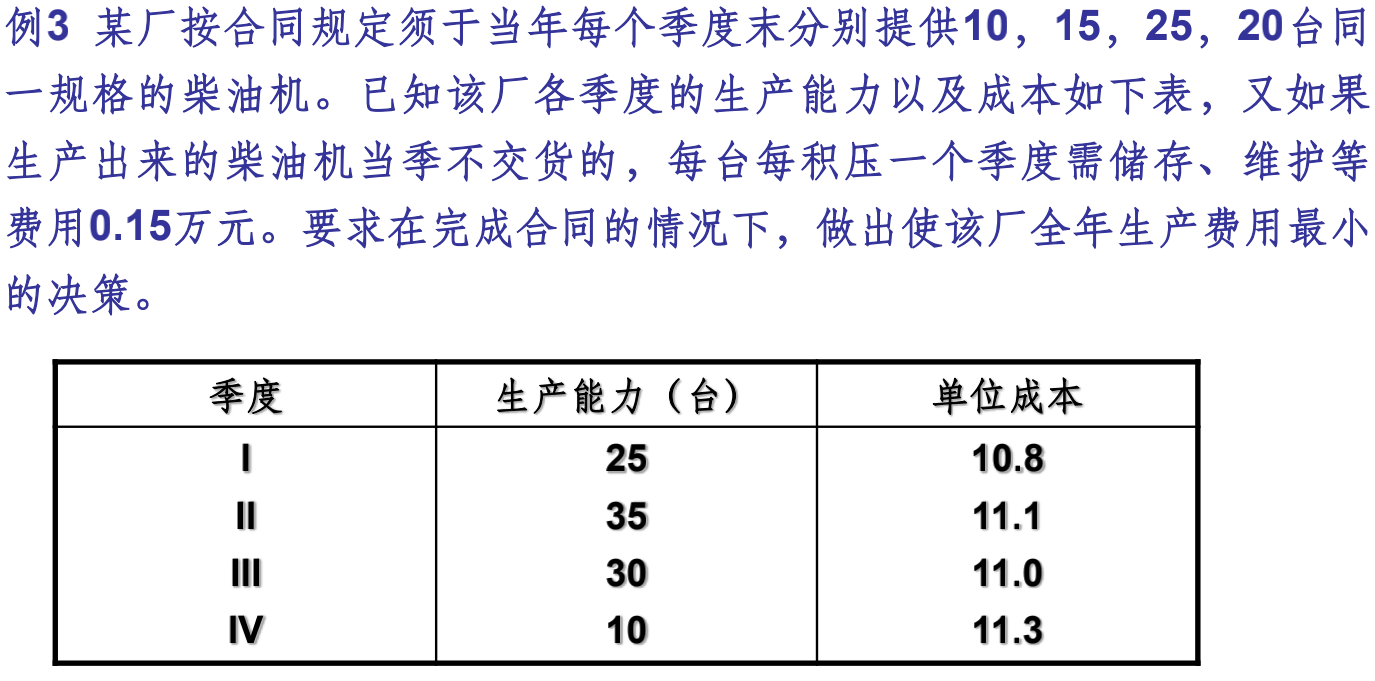
\includegraphics[scale = 0.3]{pictures/P107_Example3.png}\par
		更复杂的例子如本章例5
		\subsection{关于列出来一个供求问题}
		\indent\textsf{\textit{前方高能预警!可能会出现看到题目一脸蒙蔽,啥也列不出来的尴尬情况}}\par
		这里要说的其实不是特别多,但是很重要(\sout{废话列不出来怎么做题})。\par
		\begin{enumerate}
			\item 找出在本问题中,$\xi$要从$\mathscr{A}$到$\mathscr{B}$,这里的$\xi$指要运输的东西,$\mathscr{A}$和$\mathscr{B}$分别指这个东西从哪里来,到哪里去(人生三问?)在这里不考虑一切具体的内容,比如成本、额外成本、在不同地点之间的差别(如是否为虚设)、不同路线之间是否可到达等,但是\textit{需要把浮动部分都拆开,还有题目里面涉及到的一些额外的“固有”部分}
			\item 将所有产地销地列到一张表里面,并写出其供应量和需求量
			\item 写出对应的费用,这时候考虑题目里面涉及代价的所有内容
			\item 看看题吧,说不清了
		\end{enumerate}
	\section{线性目标规划}
		\textit{最重要的是对目标规划问题的建模}\par
		线性目标规划适用于目标函数中,决策变量具有优先级的区分的问题,即所谓多目标决策问题。线性目标规划所独有的一些特征包括:\par
		\begin{enumerate}
			\item 在决策变量之外引入正负偏差变量,分别表示决策值超过和低于目标值的部分。恰好达到:$d^++d^-$;不超过:$d^+$;不低于:$d^-$
			\item 在绝对约束之外增加目标约束条件 (目标规划特有的,可把约束右端项看作要追求的目标值,在达到目标值时允许发生正或负偏差。因此线性规划问题在约束条件或目标函数中加入正、负偏差变量可变换为目标约束)
			\item 优先因子与权系数 $P_m$
			\item 目标规划的目标函数(优先因子乘以各自的正/负偏差变量)
		\end{enumerate}\par
		另外,线性目标规划多数是求$\min z$,故检验数应非负才有满意解\par
		对于只有两个决策变量的,可以用图解法;否则需要用单纯形法(与之前不同的是,检验数分为k行,k为权重因子种数,当且仅当高优先级的检验数行均非负才考虑低优先级\par
		多重解:所有优先级检验数均非负时,存在某一个非基变量检验数均为0,则产生多重解,令这个变量为换入变量得到另一组解,这两组解的线性组合均为满意解
		\subsection{线性目标规划的重点}
		要正确理解正负偏差变量的含义,正负偏差变量是对于约束条件(等式和不等式)而言的,而不是一个决策变量的偏差值。$(-d_i^++d_i^-)$这个整体有一点人工变量 (等式)、人工变量+剩余变量,或松弛变量 (不等式) 的感觉
		\subsection{列出一个线性规划问题}
		目标函数和约束函数都有可能需要添加上正负偏差变量,作为约束条件,目标函数若存在 (具有优先级的那种) 要求,比如“利润不小于$x$",则新的目标约束为:原目标函数的$RHS\ +d^--d^+=x$,否则不在约束条范围之内,举个例子(118页\  例2):原有的约束条件$2x_1+x_2\le11$没有对应的目标要求,故为绝对约束,而其他的根据优先级写出目标函数
	\section{关于整数线性规划}
		\subsection{分支定界法}
		有一点像用二叉树来做进化算法的感觉。事实证明,适当的参考图解法可以很大的简化求解(最优解直接得出不用单纯形法了诶)(为什么我莫名想到叠加原理)\par
		建议拆分的时候写一下拆分后的区间(如果是两决策变量可以考虑画一个草图)
		\subsection{Gomory割平面法}
		基本步骤:取最优解中的一个分数值的基变量$x_i$,有 $x_i+\sum_ka_{ik}x_k=b_i$,其中 $i\in \mathbb{Q}$ (基变量下标集合),$k\in \mathbb{K}$ (非基变量下标集合);将上述等式分$[a]$和$\{a\}$移项至等号两侧,并取$RHS\le 0$为切割方程;将切割方程系数化为整数然后添加松弛变量,得到新的约束方程(\textbf{一定要先化为整数再添加松弛变量})\par
		建议把6个式子 (原等式、高斯拆分、移项、切割方程、系数化整、松弛变量) 都写一下,尤其是高斯拆分在原系数为负时很容易出错\par
		至于为什么非要让那个系数化整的方程是一个$\le\boldsymbol{b}$的形式,因为这样会添加一个松弛变量作为基变量,无需重新计算检验数(新的基变量价值系数为0)就可以之间使用对偶单纯形法了(检验数行维持LP松弛问题的可行性)
		\subsection{0-1整数线性规划}
		注意一个0-1整数线性规划另外的表述形式:
		\[\begin{cases}
			x_i\le 1\\
			x_i\ge0,\ x_i\in\mathcal{Z}
		\end{cases}\]\par
		若变量取0、1以外的非负整数,则可以用二进制计数法表示成若干个0-1变量:$x_i=\sum2^ky_k$\par
		\textit{0-1整数线性规划联想两点分布,二进制计数法联想二项分布向n重Bernoulli分布拆分的思想}\par
		一个容易被忽略的point:0-1整数线性规划问题的引入(采取方案A或方案B,采取与否方案i)\par
		隐枚举法:(以求max为例)\par
		\begin{enumerate}
			\item 添加过滤条件:观察出来的一个可行解$\underline{z}$或者隐枚举过程中计算出来的超过$\underline{z}$的$z$值,添加一个过滤条件$RHS_z=\underline{z}$
			\item 将目标函数重排,使得各决策变量的价值系数递增(求最小值则递减排列)
			\item 列表逐一枚举判断是否符合各约束条件,满足约束条件的判断$(z_i>\underline{z})\ ?\ \underline{z}=z_i\ :\ \mathtt{pass}$
		\end{enumerate}\par
		注意下面这种说法是不对的,有的约束条件不允许达到最坏的情况(如154页\ 习题6.8)\par
		【简便起见,可以直接取$\forall x_i,\ x_i=0$为初始可行解(因为一般来说排好序,算三个以内就会出现新的$\underline{z}$了)。当然,如果是求min,可选择$\forall x_i,\ x_i=1$为初始可行解,$\underline{z}$改写为$\overline{z}$即可】
		\subsection{指派问题}
		可以回忆一下图论(我不想找了太多了\textsf{0 0}),也可以想像成每个产地和销地供需量都是1,且具有整数限制的运输问题(亦即0-1运输问题)上面的只是联想理解一下,这还是有自己的简便解题方法的\dots\par
		也是类似于运输问题,必须供需平衡(即任务量=干员数量),且求最小开销\par
		匈牙利算法,依然是个人建议每一步画一个矩阵:\par
		\begin{enumerate}[label = \circled{\arabic{*}}]
			\item 利用行列变换,使各行各列都出现0
			\item 试指派
			\begin{enumerate}
				\item 从只有一个0元素的行/列开始,给这个元素画圈圈 $\circledcirc$ (或\circled{0}),同时将该列其他0划掉记为 $\varnothing$ (或 \O)
				\item 给只有一个0元素的列/行的0画圈圈,其他0划掉
				\item 重复以上两步
				\item 若剩下的所有行/列都存在多个0,则选0元素最少的行/列,标记这一行/列里面含有0元素最少的\uwave{列/行},规则如上
				\item 若 $\circledcirc$ 的个数等于矩阵阶数,则得到最优解,否则:
			\end{enumerate}
			\item 作最少直线覆盖
			\begin{enumerate}
				\item 没有 $\circledcirc$ 的行打 $\surd$
				\item 打 $\surd$ 的行中 $\varnothing$ 所在列打 $\surd$
				\item 对打 $\surd$ 的列中 $\circledcirc$ 所在的行打 $\surd$
				\item 重复2、3
				\item 没有打对勾的行和打了对勾的列划线,就得到了覆盖所有0的最少直线数
				\item 判断:若$l<n$,\texttt{goto}\ \circled{4};若\verb|(l==n)|\ \texttt{\&\&}\ $\circledcirc$的个数小于矩阵阶数,\texttt{goto}\ \circled{2},重新画$\surd$
			\end{enumerate}
			\item 调整(图论里面交错树的思想)
			\begin{enumerate}
				\item 在没有被直线覆盖的部分找到最小的元素
				\item 然后打 $\surd$ 的各行减去这个数,各列加上这个数
				\item \texttt{goto}\ \circled{2}
			\end{enumerate}
		\end{enumerate}\par
		特殊情况:多重解(最终解矩阵里面出现定点处都是$\circledcirc$或\O 的交错闭回路)、极大化(设矩阵里面最大的元素为M,取A'中的每一个元素$a_{ij}'=M-a_{ij}$)、人和任务数量不等(虚拟单位,耗时为0)、不能完成(耗时为M)
	\section{关于排队论}
		\indent\textit{这一章的公式不用记}\par
		但是要记住各个符号的含义:
		\begin{enumerate}
			\item 平均到达率:单位时间产生事件的速率 $\lambda$
			\item 平均服务率:单位时间能被服务完成的顾客数 $\mu=1/ET$
			\item 工作强度:$\rho=\frac{\lambda}{\mu}$
			\item 有效到达率:在考虑容量或者顾客源有限的情况下的实际到达率 $\lambda_{e\!f\!f}$,在 $A=B=∞$ 的情况下 $\lambda=\lambda_{e\!f\!f}$
			\item 队长:在系统中的顾客数,期望为 $L_S$
			\item 队列长:排队等待的顾客数,期望为 $L_q$
			\item 逗留时间:顾客在系统中的停留时间,期望为 $W_S$
			\item 等待时间:顾客在系统中的排队时间,期望为 $W_q$
			\item 忙期:顾客到达服务机构到服务机构再次空闲的时长
			\item 系统的状态:系统中顾客数 n
			\item 在时刻 t,系统状态为 n 的概率:$P_n(t)$
			\item 损失率 $P_N$:被拒绝排队的顾客平均数 $\lambda P_N$
		\end{enumerate}
		\subsection{关于检验分布}
		这不是概统!不需要拟合优度检验!也不需要求极大似然估计!就一阶矩估计(求期望)然后说一句差不多就行了……在分析原始数据的时候(尤其是经验分布(一般分布)):
		\begin{enumerate}
			\item 可能会用到如下4个统计量:第i号顾客到达的时间$\tau_i$,相继到达时间间隔$t_i$,服务时间$s_i$,排队时间$w_i$
			\item 有很大可能需要整理数据,对数据进行时间区段的划分,每一个区段里面一般不要小于5
			\item 计算几个指标:
			\begin{enumerate}
				\item 平均到达率:单位时间产生事件的速率 $\lambda$
				\item 平均服务率:单位时间能被服务完成的顾客数 $\mu=1/ET$
				\item 工作强度:$\rho=\frac{\lambda}{\mu}$
				\item 有效到达率:在考虑容量或者顾客源有限的情况下的实际到达率 $\lambda_{e\!f\!f}$,在 $A=B=\infty$ 的情况下 $\lambda=\lambda_{e\!f\!f}$
			\end{enumerate}
		\end{enumerate}
		\subsection{关于分析一个具体问题}
		其实就是带公式求一些指标,并可能会让分析这种情况下的策略(增加服务台,etc)。首先,像前面分析具体问题时一样,将具体问题抽象成排队论模型X/Y/Z/A/B/C,并分析其数据元素,即:写出什么是顾客、什么是服务台、排队系统里面包括哪些顾客(引出系统的状态(\textit{重点})、队长、队列长即排号数目)。然后写出来(有的题是给分布表需要求期望)到达率、服务率、工作强度$\lambda,\mu,\rho$,或者是$ET$(一般分布),然后各种代公式,\textbf{点名Little公式}。\par
		\begin{theorem}[Little Formula]
			对于任一排队系统,记$E$(服务时间)$=\dfrac1\mu$,这个排队系统若满足以下三个条件:\par
			\begin{enumerate}
				\item 排队系统能够进入统计平衡状态,即$\displaystyle\lim_{t\to\infty}P_n(t)=P(t)$
				\item 服务台的忙期与闲期交替出现,即不会一直忙着,$\rho<1$或M、N有界
				\item 系统中任一顾客不会无限等待,系统也不会永远无顾客到达,$\lambda>0,\mu>0$
			\end{enumerate}\par
			则以下Little公式总是成立的:\par
			\[L_s=W_s\lambda_e,\quad L_q=W_q\lambda_e,\quad W_s=W_q+1/\mu,\quad L_s=L_q+\lambda_e/\mu\]
		\end{theorem}
	\section{关于存储论}
		一个很基本的point是存储量随时间变化的$Q-T$函数,这个函数是锯齿状的周期函数,所考虑的即是一个周期内的各种代价最小化。锯齿的前沿可以是直线上升(生产时间很短)或者斜向上升(有生产时间);锯齿的底端可以正好在T轴上(不允许缺货)或者T轴一下(允许部分缺货)。\par
		确定性存储模型有$2\times2=4$种,其EOQ(经济批量订购)公式如下:\par
		\begin{table}[ht!]
			\centering
			\begin{tabular}{c|cc}
				\toprule
				&不允许缺货&允许缺货(缺货需补足)\\
				\midrule
				生产时间很短&$\displaystyle Q_0=\sqrt{\frac{2C_3R}{C_1}}$&$\displaystyle Q_0=\sqrt{\frac{2C_3R}{C_1}\frac{C_1+C_2}{C_2}}$\\
				生产需一定时间&$\displaystyle Q_0=\sqrt{\frac{2C_3RP}{C_1(P-R)}}$&$\displaystyle Q_0=\sqrt{\frac{2C_3R}{C_1}}\sqrt{\frac{C_1+C_2}{C_2}}\sqrt{\frac{P}{P-R}}$\\
				\bottomrule
			\end{tabular}
		\end{table}
		涉及的参数包括:
		\begin{enumerate}
			\item 订购费用 $C_3$,每一次都有,固定值
			\item 补充存储:生产批量 $Q$,生产时间 $T$,生产速度 $P$
			\item 消耗存储:需求速度 $R$,缺货损失 $C_2$,最大缺货量 $B$
			\item 存储:存储的最高数量 $S$,单位存储费 $C_1$
		\end{enumerate}\par
		基本的解题思路为:
		\begin{enumerate}
			\item 根据供求关系、模型、所需参数,列出单位时间总费用 (平均费用) 满足的方程 $C(t)$
			\item $C(t)$ 的含义是一个订货-消耗周期内,所需各种费用的平均值
			\item 求导得到极值点 $t=t_0$ (分段函数另外讨论),也就是最佳周期
			\item 由 E.O.Q 公式得到 $Q_0=R\times t_0$
		\end{enumerate}\par

	\chapter{回忆版的考试题}
		\section{2019年版}
		@printk\newline
		\textit{考完回忆的,但是一直忘了放出来,可能不全}
		\begin{enumerate}
			\item 给一个单纯型表的最后一步,求一下原来的线性规划问题的系数(倒腾倒腾式子就行)
			\item 对偶单纯形法的性质,CX <= Yb 的应用
			\item 算一个产销不平衡的运输问题
			\item 给一个整数线性规划的一步,问割平面法应该怎么加约束 \& 如果用分支定界法怎么加下一步的约束
			\item 指派问题,甲乙丙丁进行 ABCDE 五项工作,E必选,ABCD四选三
			\item 排队论 M/M/c,给了 M/M/c 和 M/M/1/N 的公式然后让你猜是哪一个
			\item 矩阵对策的图解法
		\end{enumerate}
		\section{2018年版}
		@账号已注销\newline
		\textit{根据题目序号回忆, 题目分数 10分,12分,15分}
		\begin{enumerate}
			\item 填空题,10个空10分,有单纯形法的矩阵表示,图的支撑树, 对策值等
			\item 对偶理论, 给出最优解,求一个系数的值, 然后求对偶问题的解
			\item 第一问线性规划(没有要求方法,我用的图解法),第二问目标规划, 只需要列出模型
			\item 运输问题 要求用 Vogel 得到初解
			\item 0-1规划
			\item 指派问题,5-5
			\item 最大流,最小截
			\item 对策论, 第一问求 VG, 第二问变了一个赢得矩阵, 利用对策基本定理容易求相应的对策值与对策
		\end{enumerate}

		\chapter{未知届数的笔记}
		\begin{figure}[h]
			\centering
			\includegraphics[scale = 0.1]{pictures/1.jpg}\\[10pt]
			\includegraphics[scale = 0.1]{pictures/2.jpg}
		\end{figure}
		\newpage
		\begin{figure}[h]
			\centering
			\includegraphics[scale = 0.1]{pictures/3.jpg}\\[10pt]
			\includegraphics[scale = 0.1]{pictures/4.jpg}
		\end{figure}
		\newpage
		\begin{figure}[h]
			\centering
			\includegraphics[scale = 0.1]{pictures/5.jpg}\\[10pt]
		\end{figure}
\end{document}
